%%%%%%%%%%%%%%%%%%%%%%%%%%%%%%%%%%%%%%%%%%%%%%%%%%%%%%%%%%%%%%%%%%%%%%%%%%%%%%%
% CASE STUDY TEMPLATE - Programming and Problem Solving
% Author: Brendan Shea, PhD
% Course: Programming and Problem Solving
% Rochester Community and Technical College
%%%%%%%%%%%%%%%%%%%%%%%%%%%%%%%%%%%%%%%%%%%%%%%%%%%%%%%%%%%%%%%%%%%%%%%%%%%%%%%

\documentclass[11pt,letterpaper]{article}

%---------- PACKAGES ----------%
\usepackage[margin=1in, headheight=22pt]{geometry}
\usepackage[T1]{fontenc}
\usepackage{xcolor}
\usepackage{tcolorbox}
\usepackage{graphicx}
\usepackage{titlesec}
\usepackage{enumitem}
\usepackage{fancyhdr}
\usepackage{listings}
\usepackage{hyperref}
\usepackage{multicol}
\usepackage{booktabs}
\usepackage{tikz}
\usepackage{float}
\usepackage{amssymb}
\usepackage{amsmath}
\usepackage{pifont}

% TikZ libraries
\usetikzlibrary{shapes.geometric, arrows.meta, positioning, calc, backgrounds, fit, matrix, decorations.pathreplacing, chains}

% Load tcolorbox libraries
\tcbuselibrary{skins,breakable,listings,listingsutf8}

%---------- COLOR DEFINITIONS ----------%
\definecolor{csprimary}{HTML}{2C3E50}
\definecolor{cssecondary}{HTML}{E74C3C}
\definecolor{cstertiary}{HTML}{3498DB}
\definecolor{csaccent}{HTML}{27AE60}
\definecolor{cswarm}{HTML}{F39C12}
\definecolor{cslight}{HTML}{ECF0F1}
\definecolor{csdark}{HTML}{1A252F}

% Syntax highlighting colors
\definecolor{codegreen}{HTML}{27AE60}
\definecolor{codepurple}{HTML}{9B59B6}
\definecolor{codeorange}{HTML}{E67E22}
\definecolor{codeblue}{HTML}{3498DB}
\definecolor{codegray}{HTML}{95A5A6}
\definecolor{codestring}{HTML}{E74C3C}
\definecolor{codebg}{HTML}{1E2A38}

%---------- CASE STUDY METADATA ----------%
\newcommand{\cstitle}{The Prediction Machine}
\newcommand{\cssubtitle}{How Large Language Models Work---and the Ethics of AI}
\newcommand{\csauthor}{Brendan Shea, PhD}
\newcommand{\cscourse}{Programming and Problem Solving}
\newcommand{\csinstitution}{Rochester Community and Technical College}
\newcommand{\csdate}{\today}

%---------- LISTINGS CONFIGURATION ----------%
\lstdefinestyle{basestyle}{
    backgroundcolor=\color{codebg},
    basicstyle=\ttfamily\small\color{white},
    breakatwhitespace=false,
    breaklines=true,
    captionpos=b,
    keepspaces=true,
    showspaces=false,
    showstringspaces=false,
    showtabs=false,
    tabsize=4,
    frame=none,
    xleftmargin=4mm,
    xrightmargin=4mm,
    aboveskip=0pt,
    belowskip=0pt,
}

\lstdefinestyle{javastyle}{
    style=basestyle,
    language=Java,
    keywordstyle=\color{codeblue}\bfseries,
    commentstyle=\color{codegray}\itshape,
    stringstyle=\color{codestring},
    morekeywords={String, Scanner, System, var, boolean, Math, List, Map, HashMap, ArrayList},
}

\lstdefinestyle{pythonstyle}{
    style=basestyle,
    language=Python,
    keywordstyle=\color{codeblue}\bfseries,
    commentstyle=\color{codegray}\itshape,
    stringstyle=\color{codestring},
}

%---------- CUSTOM ENVIRONMENTS ----------%
\newcommand{\keyterm}[1]{\textbf{\textcolor{cssecondary}{#1}}}

\newtcolorbox{conceptbox}[1][]{
    enhanced,
    colback=cslight,
    colframe=csprimary,
    fonttitle=\bfseries\color{white},
    title=#1,
    attach boxed title to top left={yshift=-2mm, xshift=5mm},
    boxed title style={colback=csprimary},
    breakable
}

\newtcolorbox{historybox}[1][]{
    enhanced,
    colback=codepurple!8,
    colframe=codepurple,
    fonttitle=\bfseries\color{white},
    title=#1,
    attach boxed title to top left={yshift=-2mm, xshift=5mm},
    boxed title style={colback=codepurple},
    breakable
}

\newtcolorbox{ethicsbox}[1][]{
    enhanced,
    colback=cssecondary!8,
    colframe=cssecondary,
    fonttitle=\bfseries\color{white},
    title=#1,
    attach boxed title to top left={yshift=-2mm, xshift=5mm},
    boxed title style={colback=cssecondary},
    breakable
}

\newtcolorbox{mathbox}[1][]{
    enhanced,
    colback=cstertiary!8,
    colframe=cstertiary,
    fonttitle=\bfseries\color{white},
    title=#1,
    attach boxed title to top left={yshift=-2mm, xshift=5mm},
    boxed title style={colback=cstertiary},
    breakable
}

\newtcblisting{javacode}[1][]{
    enhanced,
    colback=codebg,
    colframe=csaccent,
    colupper=white,
    fonttitle=\bfseries\color{white},
    title=#1,
    attach boxed title to top left={yshift=-2mm, xshift=5mm},
    boxed title style={colback=csaccent},
    left=0mm, right=0mm, top=2mm, bottom=2mm,
    boxrule=1pt,
    breakable,
    pad at break=2mm,
    listing only,
    listing options={style=javastyle}
}

\newtcblisting{pythoncode}[1][]{
    enhanced,
    colback=codebg,
    colframe=cstertiary,
    colupper=white,
    fonttitle=\bfseries\color{white},
    title=#1,
    attach boxed title to top left={yshift=-2mm, xshift=5mm},
    boxed title style={colback=cstertiary},
    left=0mm, right=0mm, top=2mm, bottom=2mm,
    boxrule=1pt,
    breakable,
    pad at break=2mm,
    listing only,
    listing options={style=pythonstyle}
}

\newtcolorbox{questionbox}{
    enhanced,
    colback=cswarm!10,
    colframe=cswarm,
    fonttitle=\bfseries\color{white},
    title=Discussion Questions,
    attach boxed title to top center={yshift=-2mm},
    boxed title style={colback=cswarm},
    breakable
}

\newtcolorbox{glossarybox}{
    enhanced,
    colback=cslight,
    colframe=csprimary,
    fonttitle=\bfseries\color{white},
    title=Glossary of Key Terms,
    attach boxed title to top center={yshift=-2mm},
    boxed title style={colback=csprimary},
    breakable
}

%---------- HEADER/FOOTER ----------%
\pagestyle{fancy}
\fancyhf{}
\fancyhead[L]{\small\textcolor{csprimary}{\cscourse}}
\fancyhead[R]{\small\textcolor{csprimary}{Case Study}}
\fancyfoot[C]{\thepage}
\renewcommand{\headrulewidth}{0.4pt}
\renewcommand{\headrule}{\hbox to\headwidth{\color{csprimary}\leaders\hrule height \headrulewidth\hfill}}

%---------- SECTION FORMATTING ----------%
\titleformat{\section}
    {\Large\bfseries\color{csprimary}}
    {\thesection}{1em}{}[\color{cssecondary}\titlerule]
    
\titleformat{\subsection}
    {\large\bfseries\color{cstertiary}}
    {\thesubsection}{1em}{}

%---------- HYPERLINK SETTINGS ----------%
\hypersetup{
    colorlinks=true,
    linkcolor=cstertiary,
    urlcolor=cstertiary
}

%%%%%%%%%%%%%%%%%%%%%%%%%%%%%%%%%%%%%%%%%%%%%%%%%%%%%%%%%%%%%%%%%%%%%%%%%%%%%%%
\begin{document}

%---------- TITLE BLOCK ----------%
\begin{tcolorbox}[
    enhanced,
    colback=csprimary,
    colframe=csprimary,
    arc=0mm,
    left=10mm, right=10mm, top=8mm, bottom=8mm
]
\begin{center}
    {\huge\bfseries\color{white}\cstitle}\\[3mm]
    {\Large\color{cslight}\cssubtitle}\\[5mm]
    \textcolor{cssecondary}{\rule{0.5\textwidth}{1pt}}\\[5mm]
    {\large\color{white}\csauthor}\\[2mm]
    {\normalsize\color{cslight}\cscourse\ $\bullet$ \csinstitution}
\end{center}
\end{tcolorbox}

\vspace{5mm}

%---------- INTRODUCTION ----------%
\section*{Introduction}

In November 2022, OpenAI released ChatGPT, and within two months, it had 100 million users---the fastest-growing application in history. Suddenly, anyone could have a conversation with an AI that wrote essays, explained concepts, generated code, and engaged in seemingly intelligent dialogue. The age of \keyterm{Large Language Models} (LLMs) had arrived.

But what \textit{is} ChatGPT? How can a computer program write poetry, answer questions about history, and help debug code? The answer is simultaneously simpler and more profound than most people realize. At its core, an LLM is a prediction machine: given some text, it predicts what text should come next. That's it. Yet from this simple principle emerges behavior that looks remarkably like understanding.

This case study explores how LLMs work---from the basic concepts of neural networks and training to the architecture that made modern AI possible. We'll then examine the ethical questions these systems raise: questions about bias, truth, labor, power, and what it means to create machines that mimic human thought.

\begin{conceptbox}[A Technology of Contradictions]
LLMs are simultaneously:
\begin{itemize}[leftmargin=*, itemsep=2pt]
    \item \textbf{Simple in principle}: Predict the next word
    \item \textbf{Vast in scale}: Hundreds of billions of parameters trained on trillions of words
    \item \textbf{Impressive in capability}: Write, reason, translate, code
    \item \textbf{Limited in understanding}: No true comprehension, just sophisticated pattern matching
    \item \textbf{Transformative in impact}: Reshaping education, work, and information itself
\end{itemize}
Understanding both the power and the limitations is essential for using these tools wisely.
\end{conceptbox}

%---------- BRIEF HISTORY ----------%
\section{A Brief History of Language Models}

\begin{historybox}[From ELIZA to GPT-4]
\textbf{1966}: Joseph Weizenbaum creates ELIZA, a simple chatbot that mimicked a therapist using pattern matching. Users found it surprisingly engaging despite its simplicity.

\textbf{1980s--90s}: Statistical language models emerge, calculating probabilities of word sequences from text corpora. These power early spell-checkers and speech recognition.

\textbf{2013}: Word2Vec shows that neural networks can learn meaningful word representations---words with similar meanings cluster together in mathematical space.

\textbf{2017}: Google researchers publish ``Attention Is All You Need,'' introducing the \textbf{Transformer} architecture. This breakthrough enables models to process entire sequences in parallel and track long-range dependencies.

\textbf{2018--2020}: OpenAI releases GPT (2018), GPT-2 (2019), and GPT-3 (2020), each dramatically larger than the last. GPT-3's 175 billion parameters demonstrate ``emergent'' capabilities not present in smaller models.

\textbf{2022}: ChatGPT launches, making LLMs accessible to the public. The conversational interface transforms how people interact with AI.

\textbf{2023--Present}: Rapid proliferation---GPT-4, Claude, Gemini, Llama, Mistral. LLMs become embedded in search engines, productivity tools, and countless applications.
\end{historybox}

The key insight of modern LLMs is that \textit{scale matters}. Larger models trained on more data don't just perform incrementally better---they exhibit qualitatively new capabilities. A model with 1 billion parameters might struggle with basic reasoning; one with 100 billion parameters might solve complex problems. This ``scaling law'' has driven the race to build ever-larger models.

%---------- HOW LLMS WORK ----------%
\section{How LLMs Work: The Core Ideas}

\subsection{It's All About Prediction}

Strip away the hype, and an LLM does one thing: given a sequence of text, predict what comes next. If you input ``The capital of France is,'' the model predicts that ``Paris'' is the most likely next word.

\begin{center}
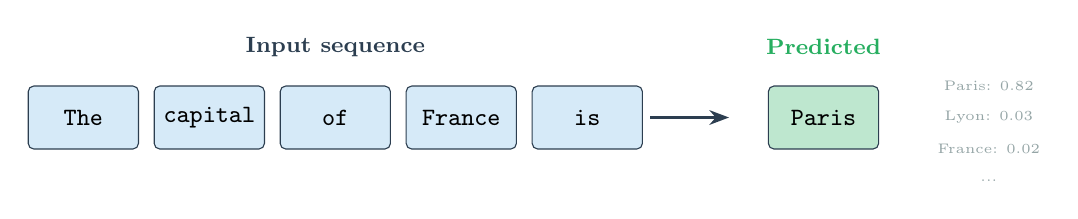
\begin{tikzpicture}[
    token/.style={rectangle, rounded corners=2pt, draw=csprimary, fill=#1, minimum width=14mm, minimum height=8mm, font=\small\ttfamily},
    arrow/.style={-{Stealth[length=2.5mm]}, thick, color=csprimary}
]

% Input tokens
\node[token=cstertiary!20] (t1) at (0,0) {The};
\node[token=cstertiary!20] (t2) at (1.6,0) {capital};
\node[token=cstertiary!20] (t3) at (3.2,0) {of};
\node[token=cstertiary!20] (t4) at (4.8,0) {France};
\node[token=cstertiary!20] (t5) at (6.4,0) {is};

% Arrow to prediction
\draw[arrow] (7.2,0) -- (8.2,0);

% Prediction with probabilities
\node[token=csaccent!30] (pred) at (9.4,0) {Paris};

% Probability distribution
\node[font=\tiny, color=codegray, align=left] at (11.5,0.4) {Paris: 0.82};
\node[font=\tiny, color=codegray, align=left] at (11.5,0) {Lyon: 0.03};
\node[font=\tiny, color=codegray, align=left] at (11.5,-0.4) {France: 0.02};
\node[font=\tiny, color=codegray, align=left] at (11.5,-0.8) {...};

% Labels
\node[font=\footnotesize\bfseries, color=csprimary] at (3.2,0.9) {Input sequence};
\node[font=\footnotesize\bfseries, color=csaccent] at (9.4,0.9) {Predicted};

\end{tikzpicture}
\end{center}

To generate longer text, the model predicts one word (actually one \keyterm{token}---more on that shortly), appends it to the input, and predicts again. A response of 100 words requires 100 sequential predictions, each building on all previous text.

\begin{javacode}[Conceptual Text Generation Loop]
public String generateText(String prompt, int maxTokens) {
    String text = prompt;
    
    for (int i = 0; i < maxTokens; i++) {
        // Get probability distribution over all possible next tokens
        Map<String, Double> probs = model.predictNext(text);
        
        // Sample from the distribution (or pick the most likely)
        String nextToken = sampleFrom(probs);
        
        // Append and continue
        text = text + nextToken;
        
        if (nextToken.equals("<END>")) break;
    }
    
    return text;
}
\end{javacode}

This simple loop---predict, append, repeat---generates everything from haikus to legal briefs. The magic lies not in the loop but in the \texttt{predictNext} function: the neural network that has learned, from trillions of words, what text typically follows what.

\subsection{Tokens: The Atoms of Language}

LLMs don't process words directly---they process \keyterm{tokens}, which are chunks of text that might be words, parts of words, or punctuation. The word ``understanding'' might be split into ``under'' + ``stand'' + ``ing.'' Common words like ``the'' are single tokens; rare words get broken into pieces.

\begin{center}
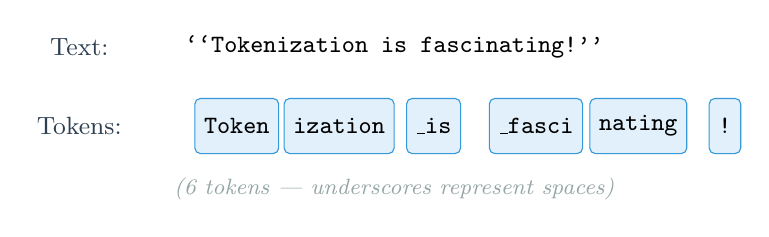
\begin{tikzpicture}[
    token/.style={rectangle, rounded corners=2pt, draw=cstertiary, fill=cstertiary!15, minimum height=7mm, font=\small\ttfamily},
]

% Tokenization example
\node[font=\small, color=csprimary] at (-2,0) {Text:};
\node[font=\small\ttfamily] at (2,0) {``Tokenization is fascinating!''};

\node[font=\small, color=csprimary] at (-2,-1) {Tokens:};
\node[token] at (0,-1) {Token};
\node[token] at (1.3,-1) {ization};
\node[token] at (2.5,-1) {\_is};
\node[token] at (3.8,-1) {\_fasci};
\node[token] at (5.1,-1) {nating};
\node[token] at (6.2,-1) {!};

\node[font=\footnotesize\itshape, color=codegray] at (2,-1.8) {(6 tokens --- underscores represent spaces)};

\end{tikzpicture}
\end{center}

Tokenization matters because it determines what the model can ``see.'' A model with a vocabulary of 50,000 tokens can represent any text as a sequence of token IDs---integers that index into the vocabulary. The model processes these numbers, not letters.

\subsection{Neural Networks: Learning Patterns}

How does the model learn to predict? Through a \keyterm{neural network}---a mathematical structure loosely inspired by the brain. A neural network consists of layers of ``neurons'' (really just numbers) connected by ``weights'' (more numbers). Input flows through the network, transformed at each layer, until output emerges.

\begin{center}
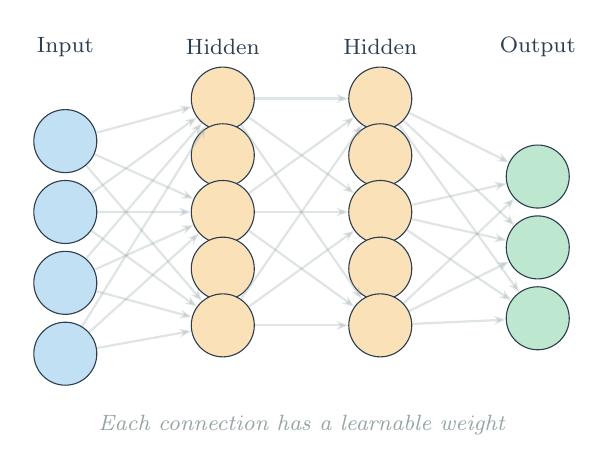
\begin{tikzpicture}[
    neuron/.style={circle, draw=csprimary, fill=#1, minimum size=8mm},
    arrow/.style={-{Stealth[length=1.5mm]}, color=codegray, thick}
]

% Input layer
\foreach \i in {1,2,3,4} {
    \node[neuron=cstertiary!30] (i\i) at (0,-\i*0.9) {};
}
\node[font=\footnotesize, color=csprimary] at (0,0.3) {Input};

% Hidden layer 1
\foreach \i in {1,2,3,4,5} {
    \node[neuron=cswarm!30] (h1\i) at (2,-\i*0.72+0.36) {};
}
\node[font=\footnotesize, color=csprimary] at (2,0.3) {Hidden};

% Hidden layer 2
\foreach \i in {1,2,3,4,5} {
    \node[neuron=cswarm!30] (h2\i) at (4,-\i*0.72+0.36) {};
}
\node[font=\footnotesize, color=csprimary] at (4,0.3) {Hidden};

% Output layer
\foreach \i in {1,2,3} {
    \node[neuron=csaccent!30] (o\i) at (6,-\i*0.9-0.45) {};
}
\node[font=\footnotesize, color=csprimary] at (6,0.3) {Output};

% Connections (subset for clarity)
\foreach \i in {1,2,3,4} {
    \foreach \j in {1,3,5} {
        \draw[arrow, opacity=0.3] (i\i) -- (h1\j);
    }
}
\foreach \i in {1,3,5} {
    \foreach \j in {1,3,5} {
        \draw[arrow, opacity=0.3] (h1\i) -- (h2\j);
    }
}
\foreach \i in {1,3,5} {
    \foreach \j in {1,2,3} {
        \draw[arrow, opacity=0.3] (h2\i) -- (o\j);
    }
}

% Label
\node[font=\footnotesize\itshape, color=codegray] at (3,-4.5) {Each connection has a learnable weight};

\end{tikzpicture}
\end{center}

During \keyterm{training}, the network sees billions of examples: given this text, the next token was X. If the network predicts wrong, the \keyterm{loss} (error) is calculated, and the weights are adjusted slightly to make that prediction more accurate next time. Repeat this billions of times, and patterns emerge: the network learns grammar, facts, reasoning styles---everything implicit in human text.

\subsection{The Transformer Architecture}

Modern LLMs use a specific neural network design called the \keyterm{Transformer}. Its key innovation is the \keyterm{attention mechanism}, which allows every token to ``attend to'' every other token in the sequence.

When processing ``The cat sat on the mat because it was tired,'' the model must understand that ``it'' refers to ``cat,'' not ``mat.'' Attention lets the model learn these connections: when processing ``it,'' the model can look back at all previous words and weight their relevance.

\begin{center}
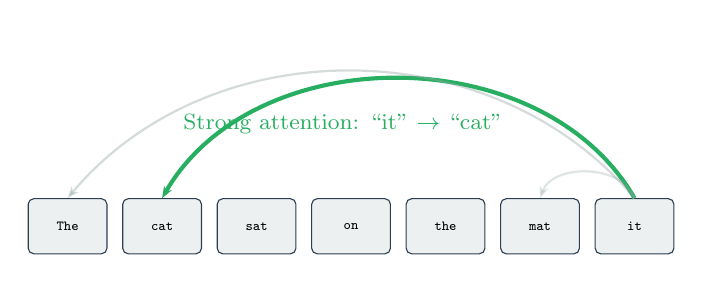
\begin{tikzpicture}[
    token/.style={rectangle, rounded corners=2pt, draw=csprimary, fill=cslight, minimum width=10mm, minimum height=7mm, font=\tiny\ttfamily},
    att/.style={-{Stealth[length=1.5mm]}, thick}
]

% Tokens
\node[token] (t1) at (0,0) {The};
\node[token] (t2) at (1.2,0) {cat};
\node[token] (t3) at (2.4,0) {sat};
\node[token] (t4) at (3.6,0) {on};
\node[token] (t5) at (4.8,0) {the};
\node[token] (t6) at (6,0) {mat};
\node[token] (t7) at (7.2,0) {it};

% Attention arrows
\draw[att, color=csaccent, line width=1.5pt] (t7.north) to[out=120, in=60] (t2.north);
\draw[att, color=codegray, opacity=0.4] (t7.north) to[out=130, in=50] (t1.north);
\draw[att, color=codegray, opacity=0.3] (t7.north) to[out=110, in=70] (t6.north);

% Label
\node[font=\footnotesize, color=csaccent] at (3.5,1.3) {Strong attention: ``it'' $\rightarrow$ ``cat''};

\end{tikzpicture}
\end{center}

Transformers process all tokens in parallel (unlike older sequential models), making them much faster to train. Multiple ``attention heads'' capture different types of relationships---some might track grammar, others semantics, others long-range dependencies. Stacking many transformer layers (GPT-4 reportedly has over 100) creates a deep network that extracts increasingly abstract patterns.

\subsection{What the Model ``Knows''}

An LLM doesn't store facts in a database---it encodes patterns in billions of numerical weights. When you ask ``What is the capital of France?,'' no lookup occurs. Instead, the network's weights have been shaped by training so that, given this input pattern, the output pattern corresponds to ``Paris.''

This is why LLMs can be confidently wrong (\keyterm{hallucinate}). They're not retrieving verified facts; they're generating text that \textit{statistically resembles} correct answers. Usually the patterns align with truth---but not always.

%---------- TRAINING AND DATA ----------%
\section{Training: Where Knowledge Comes From}

\subsection{The Training Data}

An LLM's capabilities come from its training data---the text it learned from. GPT-3 trained on roughly 500 billion tokens from sources including Common Crawl (web pages), books, Wikipedia, and code repositories. Later models use even more data.

This training data shapes everything about the model:
\begin{itemize}[itemsep=2pt]
    \item \textbf{Knowledge}: The model only ``knows'' what appeared in training data (up to its cutoff date).
    \item \textbf{Style}: It mimics the writing styles present in training.
    \item \textbf{Biases}: Biases in human text become biases in the model.
    \item \textbf{Languages}: It performs best on languages well-represented in training.
\end{itemize}

\subsection{RLHF: Teaching Models to Be Helpful}

Raw language models trained only to predict text can be erratic---they might generate toxic content, refuse to help, or produce unhelpful responses. To make models like ChatGPT useful and safe, companies use \keyterm{Reinforcement Learning from Human Feedback} (RLHF).

\begin{center}
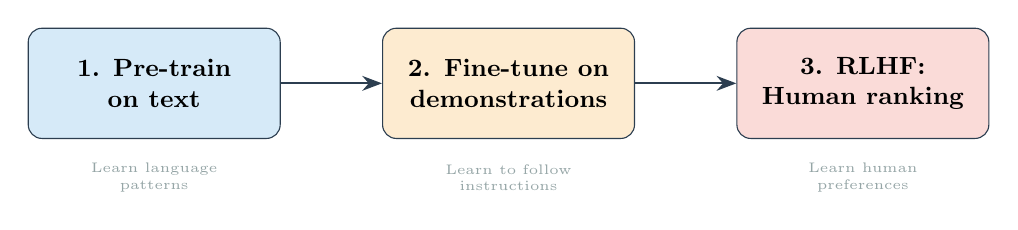
\begin{tikzpicture}[
    stage/.style={rectangle, rounded corners=5pt, draw=csprimary, fill=#1, minimum width=32mm, minimum height=14mm, font=\small\bfseries, align=center},
    arrow/.style={-{Stealth[length=2.5mm]}, thick, color=csprimary}
]

\node[stage=cstertiary!20] (s1) at (0,0) {1. Pre-train\\on text};
\node[stage=cswarm!20] (s2) at (4.5,0) {2. Fine-tune on\\demonstrations};
\node[stage=cssecondary!20] (s3) at (9,0) {3. RLHF:\\Human ranking};

\draw[arrow] (s1) -- (s2);
\draw[arrow] (s2) -- (s3);

\node[font=\tiny, color=codegray, align=center] at (0,-1.2) {Learn language\\patterns};
\node[font=\tiny, color=codegray, align=center] at (4.5,-1.2) {Learn to follow\\instructions};
\node[font=\tiny, color=codegray, align=center] at (9,-1.2) {Learn human\\preferences};

\end{tikzpicture}
\end{center}

In RLHF, human raters compare model outputs and indicate which is better. The model learns to produce responses that humans prefer---more helpful, more accurate, less harmful. This process is expensive and labor-intensive, relying on thousands of human hours.

%---------- ETHICAL ISSUES ----------%
\section{Ethical Issues in LLM Development and Deployment}

The power of LLMs brings profound ethical challenges. These aren't hypothetical future concerns---they're happening now.

\subsection{Bias and Discrimination}

LLMs learn from human-generated text, which contains human biases. Studies have found that LLMs associate certain professions with genders (``nurse'' with female, ``engineer'' with male), generate more negative sentiment for certain ethnic names, and reproduce harmful stereotypes.

\begin{ethicsbox}[Case: Bias in Image Generation]
When text-to-image systems (built on similar technology) were asked to generate images of ``a CEO,'' they overwhelmingly produced images of white men. Asked for ``a nurse,'' they produced women. These systems learned to reproduce---and arguably amplify---the biases present in their training data, including photo captions and image descriptions from the internet.
\end{ethicsbox}

The challenge is that bias is embedded in the training data itself. Debiasing techniques exist but are imperfect. And ``removing bias'' requires defining what unbiased means---a contested question.

\subsection{Hallucination and Misinformation}

LLMs confidently generate false information. They'll invent scientific citations, describe historical events that never happened, and provide plausible-sounding but incorrect technical advice. This isn't malfunction---it's inherent to how they work. They generate \textit{probable} text, not \textit{verified} text.

In high-stakes domains---medicine, law, journalism---hallucinations can cause real harm. A lawyer who submitted AI-generated legal briefs discovered the cited cases didn't exist. Medical chatbots have provided dangerous health advice. The fluent, confident style of LLM output makes hallucinations harder to detect.

\subsection{The Labor Behind the AI}

Creating ``aligned'' AI requires enormous human labor, often invisible and poorly compensated:

\begin{ethicsbox}[The Hidden Workforce]
Training data must be cleaned and labeled. RLHF requires thousands of human comparisons. Content moderation---filtering toxic outputs---exposes workers to disturbing material. Much of this work is outsourced to workers in Kenya, the Philippines, and other countries, sometimes paying less than \$2 per hour. Investigations revealed that workers screening training data for OpenAI faced traumatic content including violence and abuse.

The gleaming AI interfaces obscure this global supply chain of human labor.
\end{ethicsbox}

\subsection{Copyright and Training Data}

LLMs are trained on text scraped from the internet, much of it copyrighted: news articles, books, academic papers, personal blogs, code repositories. Authors and publishers have filed lawsuits arguing this constitutes copyright infringement.

The questions are genuinely difficult: Is training on copyrighted text ``fair use''? Can a model that has ``learned'' from a book reproduce substantial portions? If an LLM writes in a distinctive author's style (having trained on their work), who owns that output? These cases are working through courts worldwide.

\subsection{Environmental Impact}

Training large models consumes enormous computational resources---and electricity. Training GPT-3 reportedly consumed enough energy to power an average American home for over 100 years. As models grow larger and companies race to train new versions, the environmental footprint grows.

\begin{center}
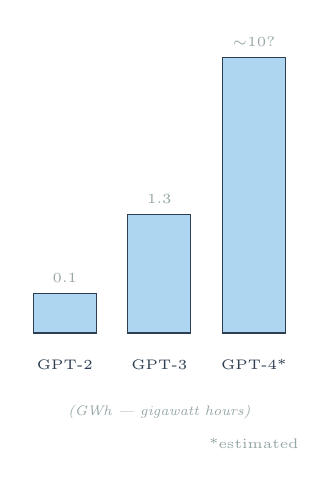
\begin{tikzpicture}[
    bar/.style={rectangle, draw=csprimary, fill=#1, minimum width=8mm},
]

% Bar chart of approximate training energy
\node[bar=cstertiary!40, minimum height=5mm] at (0,0.25) {};
\node[font=\tiny, color=csprimary] at (0,-0.4) {GPT-2};
\node[font=\tiny, color=codegray] at (0,0.7) {0.1};

\node[bar=cstertiary!40, minimum height=15mm] at (1.2,0.75) {};
\node[font=\tiny, color=csprimary] at (1.2,-0.4) {GPT-3};
\node[font=\tiny, color=codegray] at (1.2,1.7) {1.3};

\node[bar=cstertiary!40, minimum height=35mm] at (2.4,1.75) {};
\node[font=\tiny, color=csprimary] at (2.4,-0.4) {GPT-4*};
\node[font=\tiny, color=codegray] at (2.4,3.7) {$\sim$10?};

\node[font=\tiny\itshape, color=codegray] at (1.2,-1) {(GWh --- gigawatt hours)};
\node[font=\tiny, color=codegray] at (2.4,-1.4) {*estimated};

\end{tikzpicture}
\end{center}

Running inference (generating responses) also consumes energy. Every ChatGPT query uses roughly 10 times the energy of a Google search. Multiply by billions of queries, and the climate impact is significant.

\subsection{Concentration of Power}

Building frontier LLMs requires billions of dollars in compute, access to massive datasets, and teams of hundreds of researchers. Only a handful of companies---OpenAI, Google, Anthropic, Meta, a few others---can compete at the frontier. This concentrates enormous power over a transformative technology in few hands.

These companies decide what the models can and cannot do, what values they embody, and who gets access. Decisions made in San Francisco boardrooms shape how billions of people interact with information.

\subsection{Job Displacement}

LLMs can perform tasks previously requiring human expertise: writing, coding, customer service, legal research, medical triage. While technology has always displaced jobs while creating new ones, the breadth of LLM capabilities raises questions about whether this time is different.

Some jobs may transform rather than disappear---programmers using AI assistants rather than being replaced. But for workers whose skills closely match what LLMs do cheaply, the transition may be painful.

\subsection{Manipulation and Misuse}

LLMs can generate persuasive text at scale: personalized phishing emails, targeted political propaganda, fake reviews, synthetic social media personas. The same capabilities that make LLMs useful make them dangerous tools for manipulation.

Detecting AI-generated text is difficult and getting harder as models improve. A world where any text might be AI-generated undermines trust in written communication itself.

%---------- WHAT LLMS ARE NOT ----------%
\section{Open Questions and Active Debates}

The previous sections described what we know with reasonable confidence about how LLMs work. But many of the most important questions remain genuinely unsettled---debated actively by philosophers, computer scientists, and cognitive scientists. Rather than telling you what to think, this section presents the debates themselves.

\subsection{From Chatbots to Agents}

LLMs began as text generators, but they're increasingly being incorporated into \keyterm{agents}---systems that can take actions in the world. An LLM agent might browse the web, write and execute code, send emails, book appointments, or control other software. Projects like AutoGPT, LangChain agents, and Claude's computer use represent early steps toward AI systems that don't just respond but \textit{act}.

This raises new questions. A chatbot that gives bad advice is problematic; an agent that takes bad actions could cause direct harm. How much autonomy should AI agents have? What safeguards are needed? How do we maintain meaningful human oversight as agents become more capable? These are active areas of research with no consensus answers.

\subsection{Understanding, Intelligence, and Agency}

Perhaps the deepest debate concerns what LLMs \textit{are}---or aren't. Consider several positions:

\begin{conceptbox}[The Debate Over Understanding]
\textbf{The skeptical view:} LLMs are ``stochastic parrots'' (a term from researchers Emily Bender and Timnit Gebru)---sophisticated pattern-matchers that produce plausible text without any genuine understanding. They manipulate symbols without grasping meaning, like someone following Chinese translation rules without knowing Chinese (philosopher John Searle's famous ``Chinese Room'' argument).

\textbf{The moderate view:} LLMs have developed genuine but limited competencies. They've learned something real about language, reasoning, and world knowledge---but this falls short of human understanding. They might have ``functional understanding'' for specific tasks without general comprehension.

\textbf{The expansive view:} Understanding exists on a spectrum, not as binary. LLMs exhibit behaviors that, in humans, we'd attribute to understanding. Perhaps our intuitions about what ``true understanding'' requires are too restrictive, or rooted in human chauvinism. If a system can reason, explain, and apply knowledge flexibly, what more should we demand?

\textit{There is no scientific consensus.} The question may be philosophical rather than purely empirical---or it may require new concepts that don't map onto existing categories.
\end{conceptbox}

Similar debates surround \keyterm{intelligence} and \keyterm{agency}. Some argue LLMs demonstrate a form of intelligence; others insist intelligence requires embodiment, intrinsic goals, or consciousness that LLMs lack. Some see LLM-based agents as exhibiting genuine agency; others argue that without autonomous goal-formation, they remain sophisticated tools. These aren't merely semantic disputes---they affect how we should regulate AI, assign responsibility, and think about the future.

\subsection{Authorship and Creativity}

When an LLM writes a poem, who---if anyone---is the author? Consider the candidates:

\begin{itemize}[itemsep=3pt]
    \item \textbf{The human who prompted it?} They provided creative direction, but perhaps not the execution.
    \item \textbf{The LLM itself?} It generated the specific words, but can something without intentions or experiences be an ``author''?
    \item \textbf{The developers who built it?} They created the system, but didn't write this specific poem.
    \item \textbf{The authors of the training data?} The LLM's capabilities derive from their work, often used without consent.
    \item \textbf{No one / everyone?} Perhaps AI-generated content challenges our concept of authorship itself.
\end{itemize}

This matters beyond philosophy. Copyright law traditionally requires human authorship. Academic integrity policies assume individual responsibility for work. Creative communities debate whether AI art is ``real'' art. How we answer the authorship question shapes law, norms, and creative practice.

\subsection{Near-Term vs.\ Long-Term Risks}

The AI safety community itself is divided about which risks deserve priority:

\begin{ethicsbox}[Two Views on AI Risk]
\textbf{Near-term focus:} The most pressing risks are happening now: bias and discrimination in deployed systems, job displacement, misinformation at scale, concentration of power, erosion of privacy, and environmental costs. These harms are concrete, measurable, and affect real people today. Speculating about superintelligence distracts from urgent problems we can actually address.

\textbf{Long-term focus:} If AI systems become sufficiently advanced, the stakes become existential. A misaligned superintelligent AI could pose catastrophic risks---not from malevolence, but from pursuing goals that don't properly account for human values. Even a small probability of such outcomes warrants serious attention given the magnitude of potential harm.

\textbf{The tension:} Resources and attention are finite. Focusing on long-term risks might neglect current harms. Focusing only on current harms might leave us unprepared for transformative AI. Some researchers argue these concerns are complementary; others see them as competing for limited resources.
\end{ethicsbox}

Where you stand on this debate shapes views on AI governance, research priorities, and development pace. Reasonable, informed people disagree profoundly---and the stakes couldn't be higher.

%---------- USING LLMS THOUGHTFULLY ----------%
\section{Navigating Uncertainty}

Given genuine uncertainty about what LLMs are and what risks they pose, how should we approach them? Perhaps with epistemic humility:

\textbf{Verify important claims.} Whatever LLMs are, they can produce false statements. For anything consequential---facts, citations, medical or legal information---verify with authoritative sources.

\textbf{Hold conclusions lightly.} We don't fully understand these systems. Be wary of confident pronouncements---including your own---about what they can or cannot do, understand or fail to understand.

\textbf{Disclose AI involvement.} However we resolve questions of authorship, transparency matters. When AI contributes to your work, acknowledge it.

\textbf{Consider broader impacts.} Individual uses aggregate into societal effects. Training data, labor practices, environmental costs, and automation effects connect your choices to larger systems.

\textbf{Engage with the debates.} The questions in this case study don't have settled answers. Form your own views through reflection and discussion---but remain open to evidence and argument. The conversation is just beginning.

%---------- DISCUSSION QUESTIONS ----------%
\section*{Discussion Questions}

\begin{questionbox}
\begin{enumerate}[leftmargin=*, label=\textcolor{cswarm}{\textbf{\arabic*.}}]
    \item \textbf{The Understanding Debate:} You've seen three positions on whether LLMs ``understand'': skeptical (stochastic parrots), moderate (limited functional understanding), and expansive (understanding on a spectrum). Which view do you find most compelling, and why? What evidence or argument might change your mind?

    \item \textbf{Agents and Autonomy:} As LLMs are incorporated into agents that can take real-world actions, what level of autonomy is appropriate? Should an AI agent be able to send emails on your behalf? Make purchases? What safeguards would you want, and who should design them?

    \item \textbf{Authorship and Creativity:} If you use an LLM to help write an essay, who is the author? Does it matter whether the LLM wrote 10\% or 90\%? How should academic integrity policies, copyright law, and creative norms adapt to AI-assisted work?

    \item \textbf{Risk Priorities:} The AI safety community debates whether to prioritize near-term harms (bias, job loss, misinformation) or long-term risks (misaligned superintelligence). Where do you think attention and resources should focus? Can both be addressed simultaneously, or must we choose?

    \item \textbf{Your Own Position:} After reading this case study, what's your overall view of LLMs? Are they powerful tools, emerging minds, dangerous technologies, overhyped products, or something else entirely? What uncertainties remain in your thinking?
\end{enumerate}
\end{questionbox}

%---------- GLOSSARY ----------%
\section*{Key Terms}

\begin{glossarybox}
\begin{description}[leftmargin=!, labelwidth=3.4cm, font=\bfseries\color{cssecondary}]
    \item[Agent] An AI system that can take actions in the world (browsing, coding, sending messages), not just generate text.
    
    \item[Agency] The capacity to act autonomously toward goals---whether LLMs or LLM-based systems possess genuine agency is debated.
    
    \item[Attention Mechanism] A technique allowing neural networks to weigh the relevance of different parts of input when processing each token.
    
    \item[Embedding] A vector of numbers representing a token's meaning, learned during training to capture semantic relationships.
    
    \item[Hallucination] When an LLM generates plausible-sounding but factually false information---an inherent risk of prediction-based systems.
    
    \item[Intelligence] The capacity for reasoning, learning, and problem-solving---whether LLMs exhibit genuine intelligence remains contested.
    
    \item[Large Language Model] A neural network with billions of parameters trained on massive text data to predict and generate language.
    
    \item[Neural Network] A computational model with layers of connected nodes whose connection strengths (weights) are learned from data.
    
    \item[RLHF] Reinforcement Learning from Human Feedback; training models to produce outputs that humans rate as preferable.
    
    \item[Stochastic Parrot] A critical term suggesting LLMs merely produce statistically likely text without genuine understanding.
    
    \item[Token] A unit of text (word, subword, or punctuation) that serves as input and output for language models.
    
    \item[Training] The process of adjusting neural network weights by exposure to billions of examples to minimize prediction error.
    
    \item[Transformer] The neural network architecture underlying modern LLMs, using attention mechanisms and parallel processing.
    
    \item[Understanding] Grasping meaning and implications---whether LLMs possess any form of understanding is actively debated.
\end{description}
\end{glossarybox}

\vspace{5mm}

%---------- FOOTER ----------%
\begin{center}
\textcolor{csprimary}{\rule{0.6\textwidth}{0.5pt}}\\[3mm]
{\small\textcolor{gray}{This case study is part of the Open Educational Resources for \cscourse.\\
Licensed under Creative Commons Attribution 4.0 (CC BY 4.0).}}
\end{center}

\end{document}